\section{RESULTS}
\label{sec:result}

\subsection{Analysis Method}
\label{subsec:analysis}


Because each participant contributed three sessions, session-level records are not independent. Between-group contrasts were computed on participant-level means over the three games ($n=16$ per group) with Welch's $t$-test; within-participant contrasts across games used paired $t$-tests. Convergent validity between speech-derived and self-reported IPQ scores was quantified with Pearson's $r$ and Spearman's $\rho$ at the session level, the participant level, and on within-participant deviation scores (each participant's own mean removed), which isolate variation across games within the same person. Because the pipeline's final anchoring and aggregation rules were selected on the first seven participants (21 sessions) using agreement with self-report as one criterion, those participants form a development sample; the remaining nine (27 sessions) were scored after the pipeline was frozen and serve as a held-out confirmation sample. The primary convergence estimate is reported on the held-out sample with participant-clustered bootstrap confidence intervals (5{,}000 resamples of participants); the development sample and the pooled 48 sessions are reported alongside.

The primary evaluation unit for the speech-derived IPQ is the total score, following the IPQ reporting guideline~\cite{tran2024ipq} and our own coverage findings: INV is the least covered subscale and its within-participant correlation is null (Sections~\ref{subsec:sample} and~\ref{subsec:rq1_convergence}). Subscale results are complementary, not parallel primary indicators. Within-person agreement for the total (Section~\ref{subsec:rq1_within}) was assessed against a chance baseline from randomly re-assigning the speech-derived scores across the same participant's three games ($20{,}000$ permutations); binomial $p$ values are reported for comparison and yield the same conclusions.

Familywise error across the five group-comparison measures was controlled with the Holm--Bonferroni procedure; uncorrected and corrected $p$ values are both reported, and asterisks in tables mark uncorrected $p<.05$ only. Effect sizes are Cohen's $d$, with Hedges' $g$ and its 95\% CI for the primary group contrast; classification recall carries Wilson 95\% CIs. Missing values were left missing, and the significance level was 5\%.

Because a non-significant level difference is not evidence of agreement, the level comparison between speech-derived and self-reported totals was complemented with equivalence testing (TOST~\cite{lakens2017equivalence,lakens2018tutorial}), as used earlier in VR measurement studies~\cite{lee2012equivalence,sanaei2024scene,johnsdorf2025memory}. No consensus margin exists for the IPQ, so the primary margin was the smallest detectable change derived from the questionnaire's own $SEM$ ($\alpha=.87$~\cite{schwind2019presence} in VR settings; $SD$ from the full 32-participant sample), with sensitivity analyses under three alternative rules ($1.96\,SEM$, own-sample $\alpha$, TAP-only $SD$). Equivalence tests were run at the participant level ($n=16$). Individual-level agreement was quantified with Bland--Altman limits of agreement~\cite{bland1986statistical} and Lin's concordance correlation~\cite{lin1989concordance}, because equivalence of means does not imply interchangeability of individual scores.

An INV-side calibration term ($+0.5535$, the observed INV level offset) is reported alongside the uncorrected numbers in Section~\ref{subsec:rq1_convergence}; it is not applied to the primary indicator, and the direction and rank analyses use the uncalibrated indicator throughout.


\subsection{Sample and Data Coverage}
\label{subsec:sample}

Self-reported IPQ scores were available for all 96 sessions. Speech-derived IPQ scores exist only for the TAP group, where the pipeline produced a primary-indicator score for all 48 sessions from a total of 3{,}595 utterances (\textit{M} $=74.90$ utterances per session, \textit{SD} $=25.33$). The non-TAP group produced no think-aloud data by design, so all speech-based analyses below are restricted to the TAP group.

Coverage was uneven at the item level (Figure~\ref{fig:missing_items}). Across the 48 TAP sessions, a mean of 9.54 of the 14 IPQ items ($SD=2.00$, $Mdn=10$, range 5--13) carried at least one piece of supporting evidence; no session had all 14 items covered, and five sessions covered fewer than seven. Item-level gaps were concentrated in the involvement subscale: INV1 was uncovered in 46 of 48 sessions (95.8\%), INV3 in 43 (89.6\%), and INV2 in 31 (64.6\%), followed by REAL4 in 26 (54.2\%). The remaining ten items were uncovered in 14 or fewer sessions each. In total, 214 item slots were uncovered, a mean of 4.46 per session.

\paragraph{Reliability of the reference instrument.}
The self-reported IPQ served as the reference against which the speech-derived score is evaluated, so its own reliability bounds how closely any second measure can be expected to track it. Computed on participant-level item means over the three games ($n=32$), Cronbach's $\alpha$ for the 14-item total was $.816$, in the range reported for the IPQ in VR studies ($\alpha=.87$~\cite{schwind2019presence}); the subscales were less consistent (SP $.741$, INV $.714$, REAL $.684$; GP is a single item). Corrected item--total correlations ranged from $.129$ (INV1) to $.776$ (INV4); INV1, the item least covered by speech (Section~\ref{subsec:sample}), was also the item most weakly bound to the questionnaire total. Reliability differed by group in one subscale: the SP subscale was consistent in the non-TAP group ($\alpha=.869$) but not in the TAP group ($\alpha=.191$), while the totals were comparable (non-TAP $.829$, TAP $.700$). With 16 participants per group this contrast is fragile, and we treat it as a hypothesis about the protocol's effect on spatial-presence self-report, not as a finding (Section~\ref{subsec:rq3}).


\begin{figure}[t]
\centering
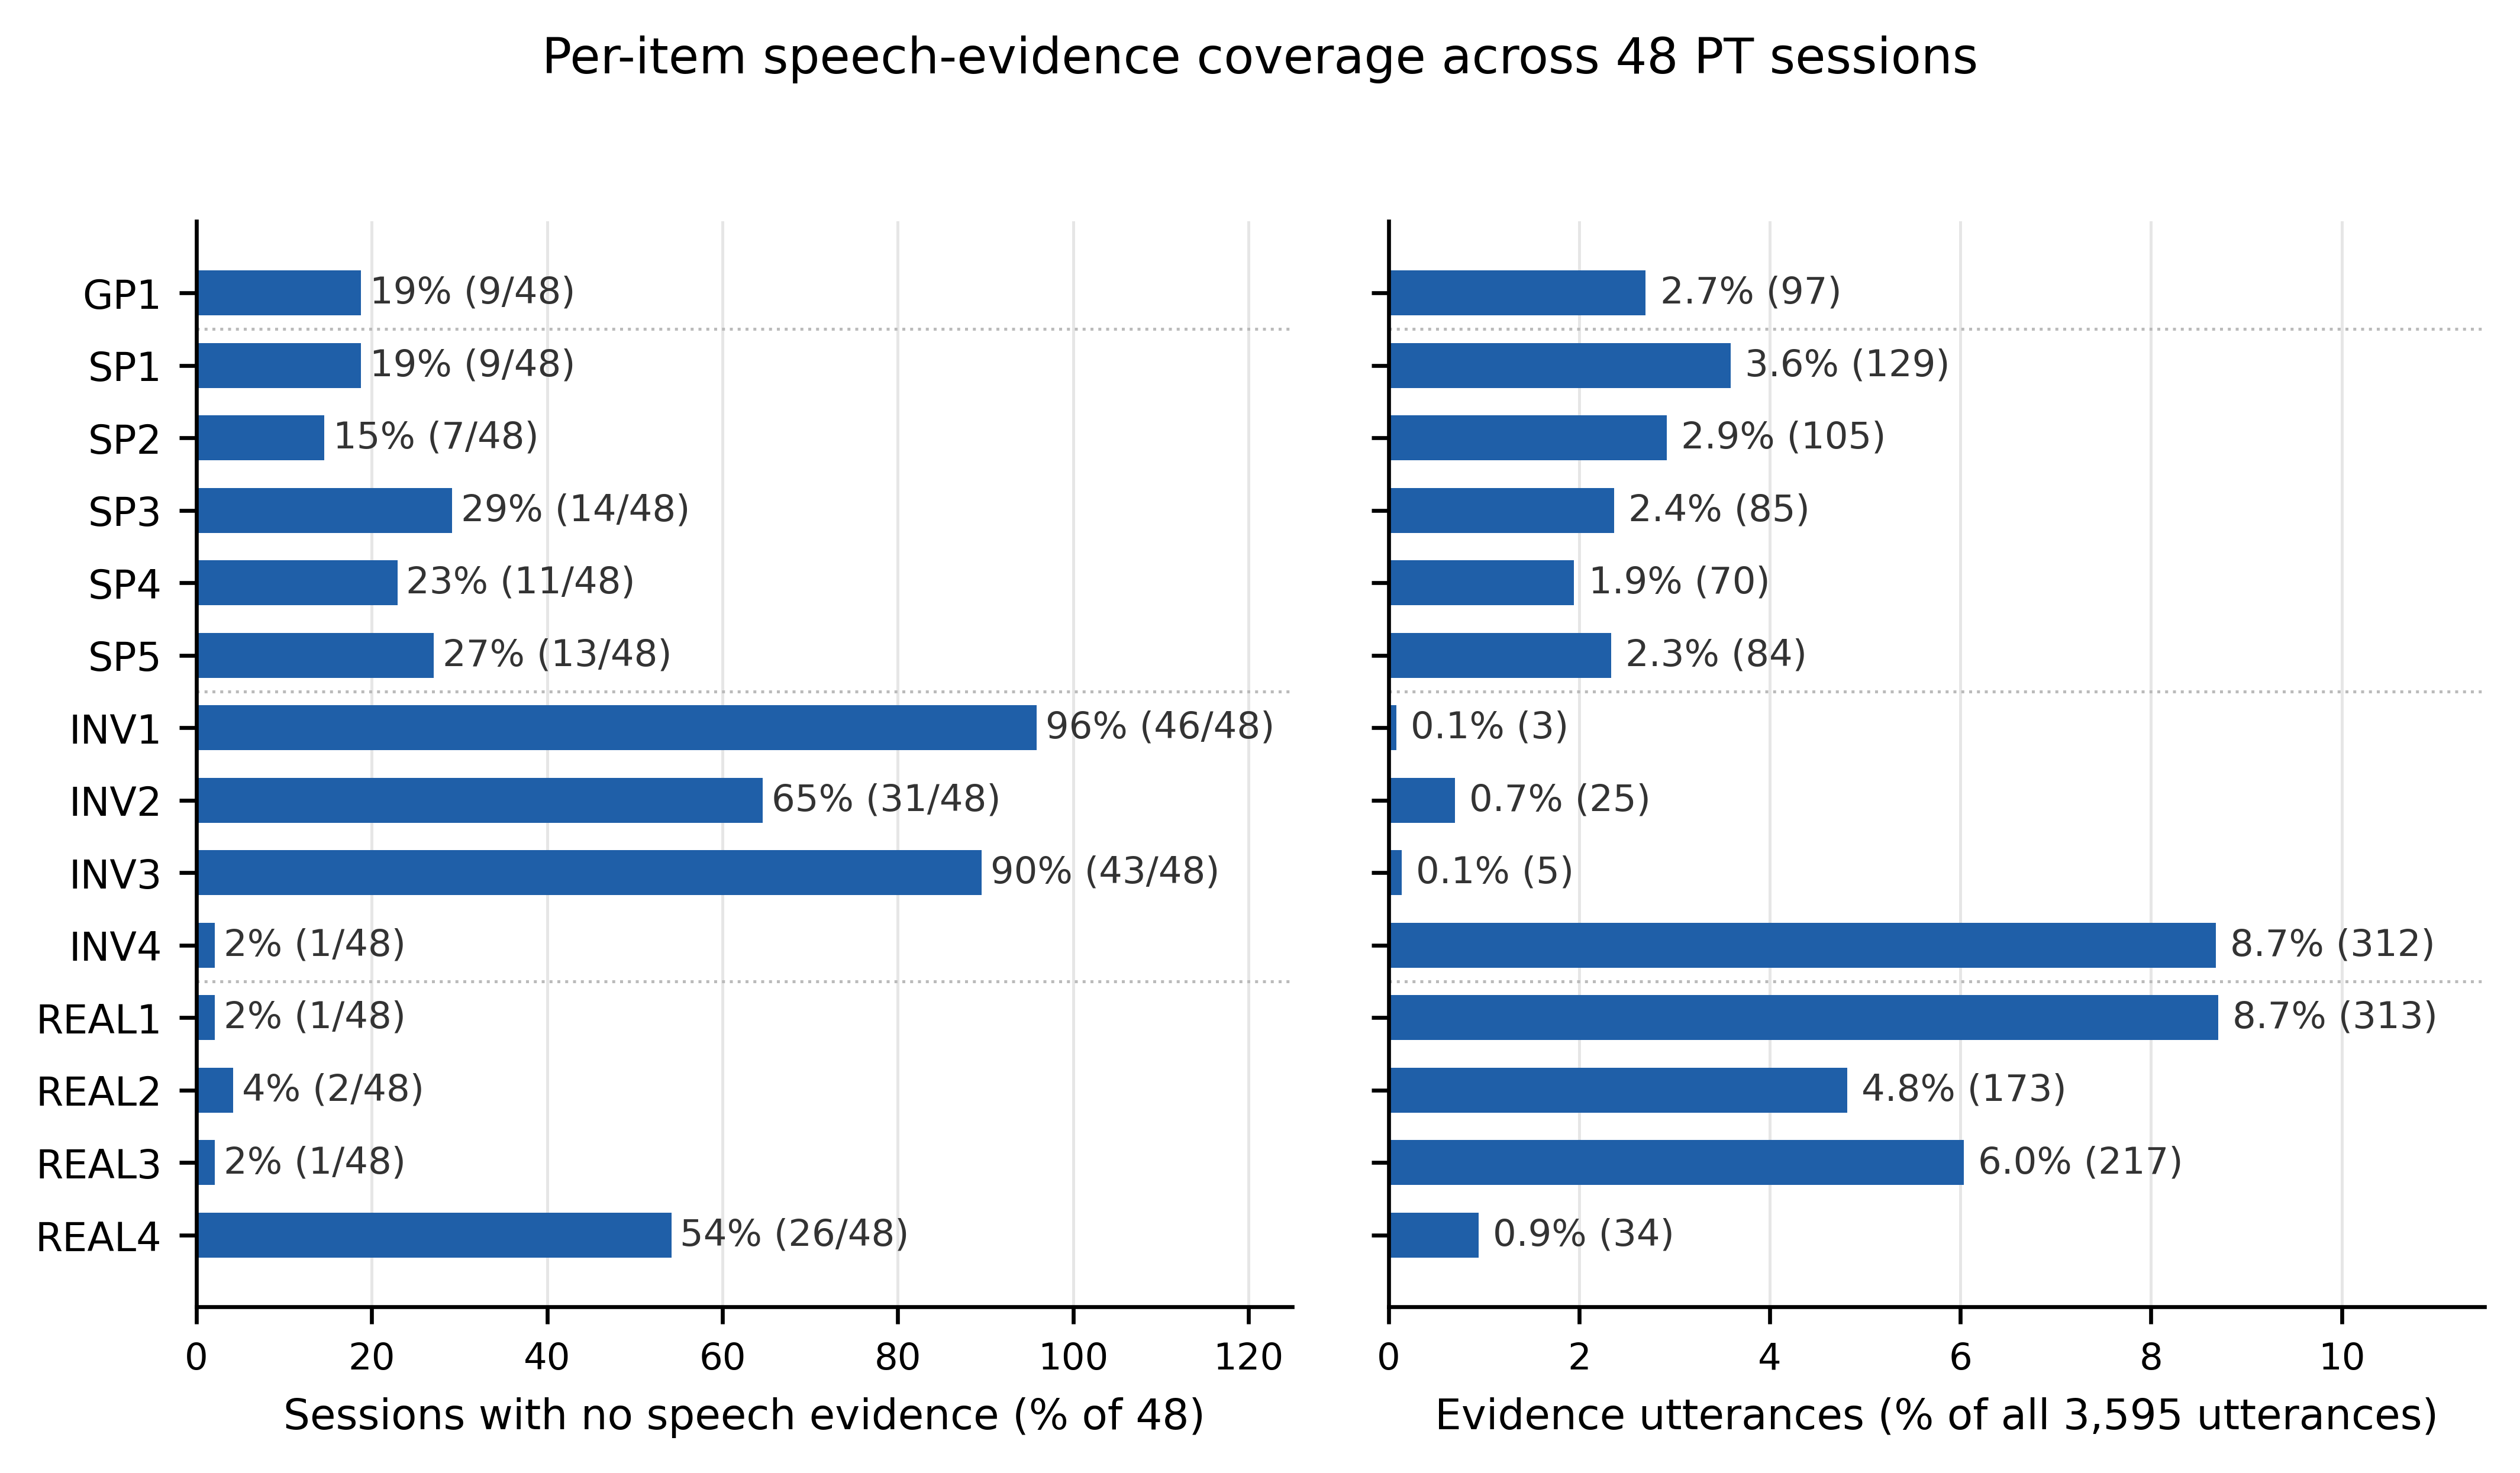
\includegraphics[width=0.85\linewidth]{Figures/F04b_item_coverage.png}
\caption{Per-item speech-evidence coverage across the 48 TAP sessions. Left: share of sessions in which the item received no speech evidence. Right: evidence utterances per item as a share of all 3{,}595 utterances (counts in parentheses; an utterance can support more than one item, so shares do not sum to 100\%). INV1 and INV3 were supported by 3 and 5 utterances in total, whereas INV4 and REAL1 each drew over 300.}
\label{fig:missing_items}
\Description{Bar chart of uncovered-session counts per IPQ item, with INV1, INV3, and INV2 leading.}
\end{figure}


\subsection{RQ1a: Within-Person Agreement in Presence Direction Across VR Games}
\label{subsec:rq1_within}

The primary RQ1 test is the held-out convergence reported in Section~\ref{subsec:rq1_convergence}; this section reports the secondary within-person indicators, which ask whether the speech-derived IPQ total tracks the direction of a participant's own presence differences across the three VR games. Table~\ref{tab:within_person} reports three within-person agreement rates against their chance baselines, with permutation and binomial $p$ values.

Within a participant, the speech-derived total picked the participant's own highest-presence game (top-1) in $11$ of $16$ cases (\textbf{69\%}) against a chance baseline of $33\%$. Considering the three ordered pairs a participant contributes (with ties on the questionnaire excluded), the speech-derived total agreed with the survey on the direction of $35$ of $46$ pairs (\textbf{76\%}) against a chance baseline of $50\%$. The complete three-game rank matched in $5$ of $16$ cases ($31\%$), above the chance baseline of $17\%$ but not statistically distinguishable from chance at the current sample size. The mean per-participant Spearman correlation between speech and survey rankings across the three games was $\rho=0.59$. Figure~\ref{fig:within_participant_profiles} shows each participant's three-game profile under both measures.

\begin{table}[t]
\centering
\caption{Within-participant agreement between speech-derived and self-reported IPQ total across the three VR games ($n=16$). Chance baselines assume random re-assignment of the speech scores among the same participant's three games. The permutation test re-assigns speech scores across the same participant's three games ($20{,}000$ permutations) and is the primary reference; the binomial test is included for comparison.}
\label{tab:within_person}
\small
\begin{tabular}{lcccc}
\hline
Indicator & Observed & Chance & $p_{\mathrm{perm}}$ & $p_{\mathrm{binom}}$ \\
\hline
Top-1 game match & $11/16 = 69\%$ & $33\%$ & $.0037$ & $.0040$ \\
Pairwise direction match & $35/46 = 76\%$ & $50\%$ & $.0006$ & $.0003$ \\
Complete 3-game rank match & $5/16 = 31\%$ & $17\%$ & n/a & $.1134$ \\
Mean per-participant Spearman $\rho$ & $0.59$ & $0$ & --- & --- \\
\hline
\end{tabular}
\end{table}

Table~\ref{tab:within_by_construct} in Appendix~\ref{sec:appendix} shows the same within-person indicators computed on the four subscales. INV shows a within-person top-1 rate of $73\%$ that comes with a null within-person correlation (Section~\ref{subsec:rq1_convergence}), consistent with the interpretation that the subscale rank is dominated by a few sessions in which any INV evidence was found at all; the total score is the more robust indicator on the current sample.


Two observations on the direction indicators of the total. First, when the pipeline missed the top-1 game (5 of 16 cases), the disagreement was concentrated on a single game contrast: in every one of the five cases the questionnaire's top game was Alyx and the pipeline's top game was Subside; Subside was the pipeline's top game for $12$ of $16$ participants and the questionnaire's top game for $8$ of $16$. Second, The Lab was near-uniformly the lowest-presence game (questionnaire $13/16$, pipeline $11/16$), so most of the within-person signal lives in the Alyx--Subside contrast.

Between-participant rank agreement was smaller than within-participant agreement: ranking the sixteen participants by their three-game mean, the Spearman correlation between speech-derived and self-reported ranks was $\rho=0.49$. We therefore read the total-score result primarily at the within-person level.


\begin{figure*}[t]
\centering
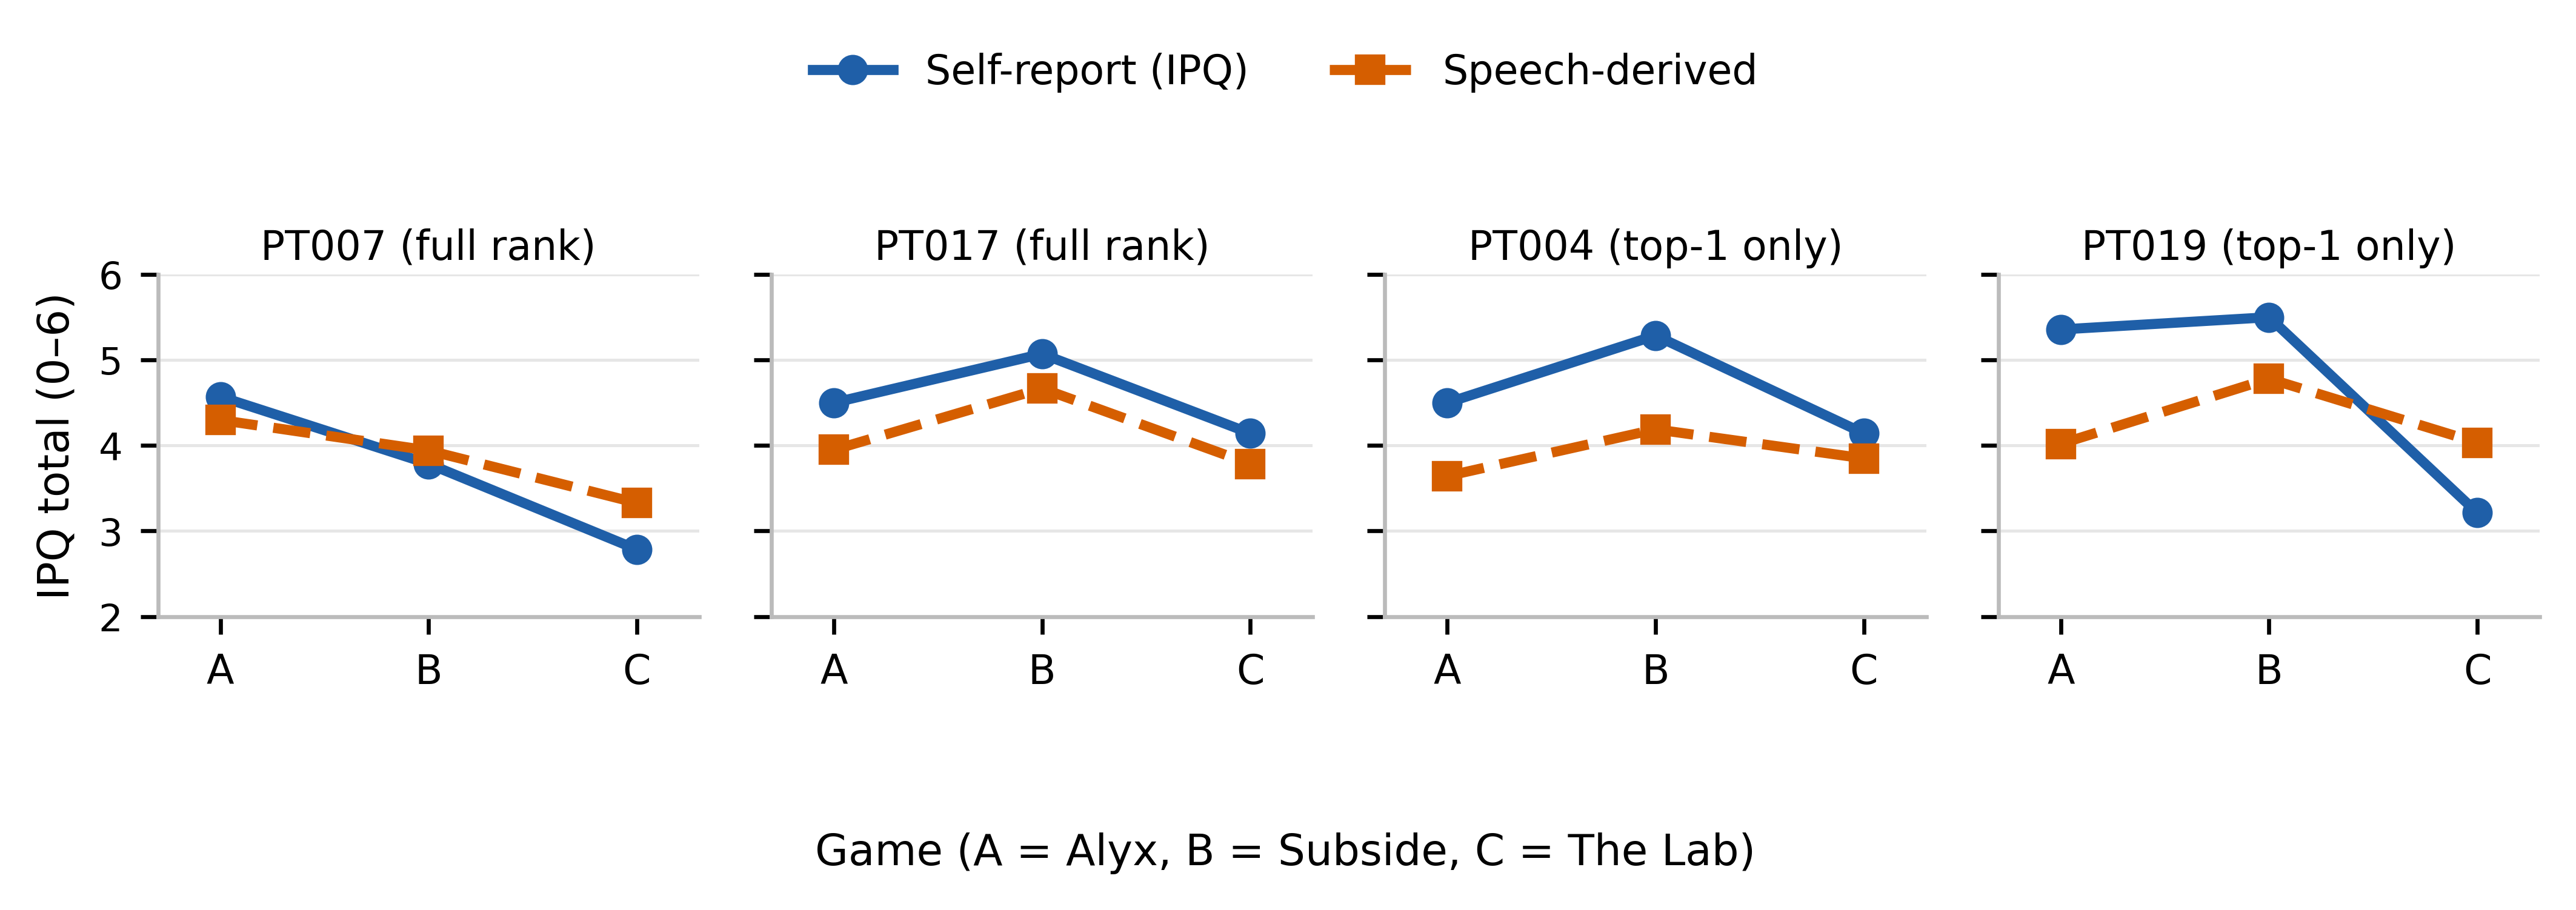
\includegraphics[width=\textwidth]{Figures/F11_within_participant_profiles.png}
\caption{Within-participant three-game profiles of the IPQ total for four participants, selected as two whose three-game rank the speech score reproduced in full and two for which only the highest-presence game matched. Within each panel the three VR games sit on the horizontal axis and the IPQ total ($0$--$6$) on the vertical axis; the self-reported score is a solid line with circular markers and the speech-derived score a dashed line with square markers. Across all 16 participants the speech-derived total matched the direction of $35/46 = 76\%$ of ordered game pairs (permutation $p=.0006$), picked the participant's own highest-presence game in $11/16 = 69\%$ of cases (permutation $p=.004$), and reproduced the complete three-game rank in $5/16 = 31\%$ of cases (n.s.).}
\label{fig:within_participant_profiles}
\Description{Four per-participant panels in one row showing speech-derived and self-reported IPQ totals across the three VR games, with panel titles indicating full rank or top-1 only.}
\end{figure*}


Because every rated item carries the timestamp of the utterance that supplied its evidence, the interface also replays how a session score was reached. Figure~\ref{fig:trajectory} shows the same four participants' sessions as they accumulated. Recomputing from the complete evidence returns the reported session score for 240 of 240 session-by-index values across the 48 sessions (agreement within $0.002$), so the replay and the reported score are one quantity read at different times; across those sessions the total moved a median of $1.01$ points over a whole session and $0.24$ points over its second half.

\begin{figure*}[t]
\centering
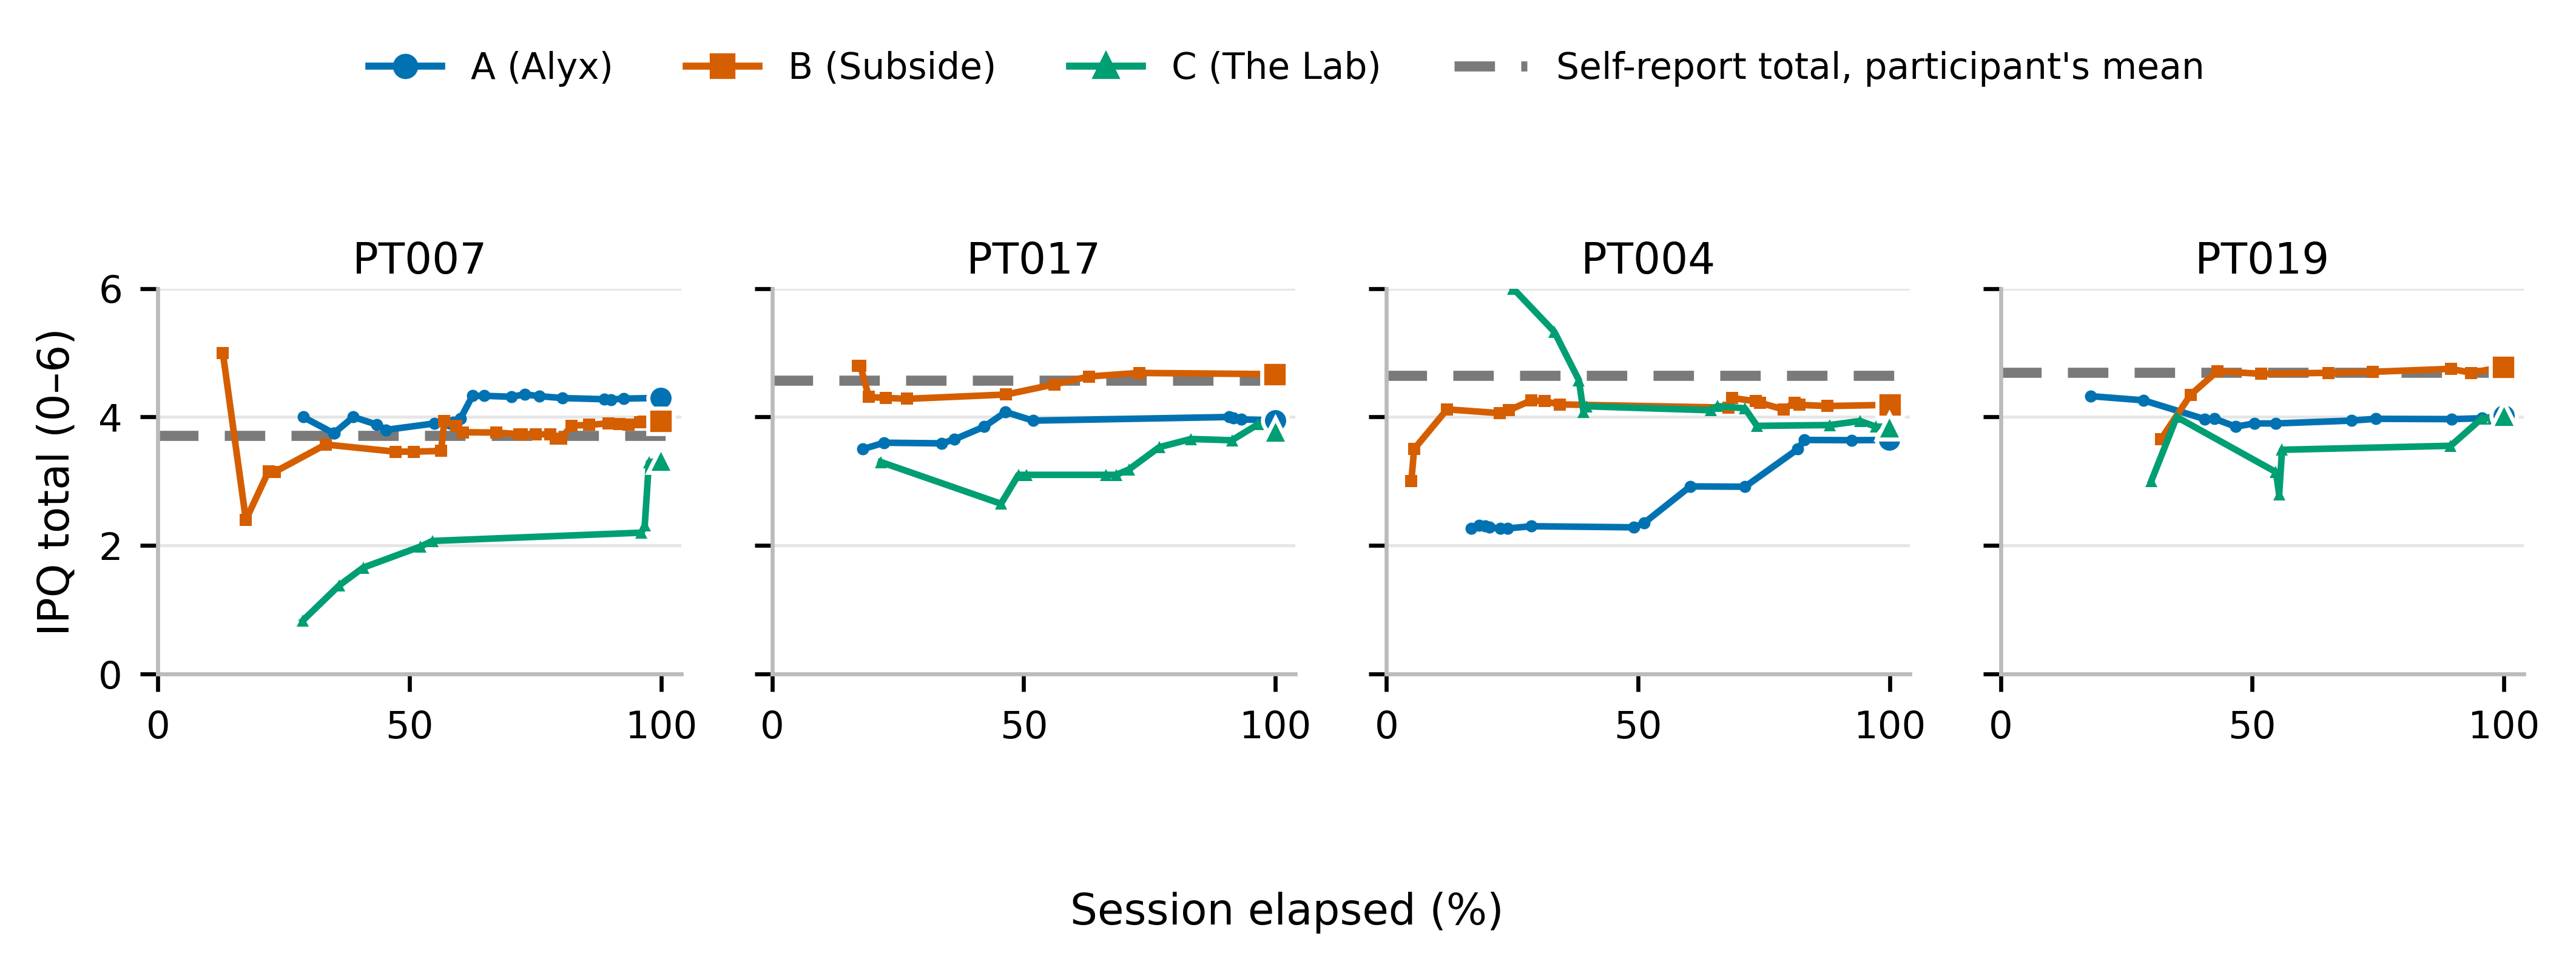
\includegraphics[width=\textwidth]{Figures/F13_score_trajectory.png}
\caption{Speech-derived IPQ total accumulating through each session, shown for four participants with one line per VR game. Each point recomputes the evidence-gated score from all item evidence available up to that moment, using the aggregation applied to the session score. The filled marker ending each line is the session score reported in the results. The grey dashed line is the participant's mean self-reported total across the three sessions, shown as a single reference; the per-game comparison of speech-derived and self-reported scores is given in Figure~\ref{fig:within_participant_profiles}. Sessions carried a median of 14 evidence utterances (range 8 to 55), so the earliest points rest on one or two items.}
\Description{Four small panels side by side, one per participant. Each panel plots three cumulative score lines, one per VR game, against percentage of session time elapsed, with filled end markers and a single grey dashed reference line.}
\label{fig:trajectory}
\end{figure*}

\subsection{RQ1b: Convergence and Level Offset}
\label{subsec:rq1_convergence}

On the held-out confirmation sample (9 participants, 27 sessions), the speech-derived IPQ total correlated moderately to strongly with the self-reported total ($r=+.608$, $p=.0008$; participant-clustered bootstrap 95\% CI $[+.26, +.85]$; $\rho=+.615$, $p=.0006$). The association held at the participant level (three-session means, $r=+.818$, $n=9$, $p=.007$) and within participants after removing individual means ($r=+.469$, $p=.014$). Session-level intraclass correlation of the questionnaire total was low ($\mathrm{ICC}=.09$), so the 27 sessions correspond to roughly 23 effectively independent observations. The development sample, on which the pipeline had been selected, showed a weaker and non-significant association ($r=+.285$, $p=.21$, $n=21$), and the pooled 48 sessions fell between the two ($r=+.419$, $p=.003$; clustered CI $[+.20, +.67]$). Applying the INV calibration constant Applying the INV calibration constant (Table~\ref{tab:calibration_prepost} in Appendix~\ref{sec:appendix}) left the held-out correlation significant but lower ($r=+.525$, $p=.006$); because that constant was estimated on all 47 scored sessions, uncalibrated scores are reported as primary.

\begin{table}[t]
\centering
\caption{Held-out, development, and pooled convergence of the speech-derived IPQ total with the self-report, on the same 16 TAP participants split by whether they were used to select the pipeline.}
\label{tab:heldout_convergence}
\small
\begin{tabular}{lcccccc}
\hline
Sample & Participants & Sessions & $r$ & $p$ & Clustered 95\% CI & $\rho$ \\
\hline
Held-out & 9 & 27 & $+.608$ & $.0008$ & $[+.26,\ +.85]$ & $+.615$ \\
Development & 7 & 21 & $+.285$ & $.21$ & --- & --- \\
Pooled & 16 & 48 & $+.419$ & $.003$ & $[+.20,\ +.67]$ & --- \\
\hline
\end{tabular}
\end{table}

For reference, Table~\ref{tab:convergence} in Appendix~\ref{sec:appendix} reports the correlation between the speech-derived IPQ score and the self-reported IPQ score at the three levels of aggregation on the pooled sample (16 participants, 48 sessions). At the session level the total score converged at $r=+.419$ ($p=.003$), and the rank-based estimate was of comparable size ($\rho=+.461$, $p=.001$). Aggregating to participant means raised the point estimate but widened the interval implied by the smaller sample ($r=+.488$, $p=.055$, $n=16$). The within-participant estimate, which asks whether a participant's speech scores rise and fall across games in step with that participant's own questionnaire responses, was $r=+.386$ ($p=.007$).

The subscales diverged sharply. On the within-participant estimate, REAL ($r=+.418$, $p=.003$), GP ($r=+.416$, $p=.009$), and SP ($r=+.293$, $p=.046$) all showed positive convergence, whereas INV was effectively zero and slightly negative ($r=-.055$, $p=.715$). Per-construct, per-level correlations with their confidence intervals are given in Table~\ref{tab:convergence}.


Convergence in rank order was accompanied by a systematic offset in level. Comparing the two scores within the same session (Table~\ref{tab:levelbias}, Figure~\ref{fig:bland_altman}), the speech-derived total score sat below the self-reported total by $-0.232$ points on the $0$--$6$ scale ($t(47)=-2.286$, $p=.027$, $d=-0.330$). The offset was largest for INV ($-0.554$, $p=.003$, $d=-0.456$) and present for SP ($-0.245$, $p=.041$), while GP ($+0.010$, $p=.940$) and REAL ($-0.005$, $p=.975$) showed no offset.

\begin{table}[t]
\centering
\caption{Level offset between the speech-derived and self-reported IPQ scores within the same session (speech $-$ survey), TAP group. Asterisks mark uncorrected $p<.05$.}
\label{tab:levelbias}
\small
\begin{tabular}{lccccc}
\hline
Scale & $n$ & $M$ diff & $SD$ & $t$ & $p$ \\
\hline
Total & 48 & $-0.232$ & $0.703$ & $-2.286$ & $.027$* \\
GP & 39 & $+0.010$ & $0.845$ & $+0.076$ & $.940$ \\
SP & 47 & $-0.245$ & $0.799$ & $-2.098$ & $.041$* \\
INV & 47 & $-0.554$ & $1.213$ & $-3.128$ & $.003$* \\
REAL & 48 & $-0.005$ & $1.101$ & $-0.031$ & $.975$ \\
\hline
\end{tabular}
\end{table}

\begin{figure*}[t]
\centering
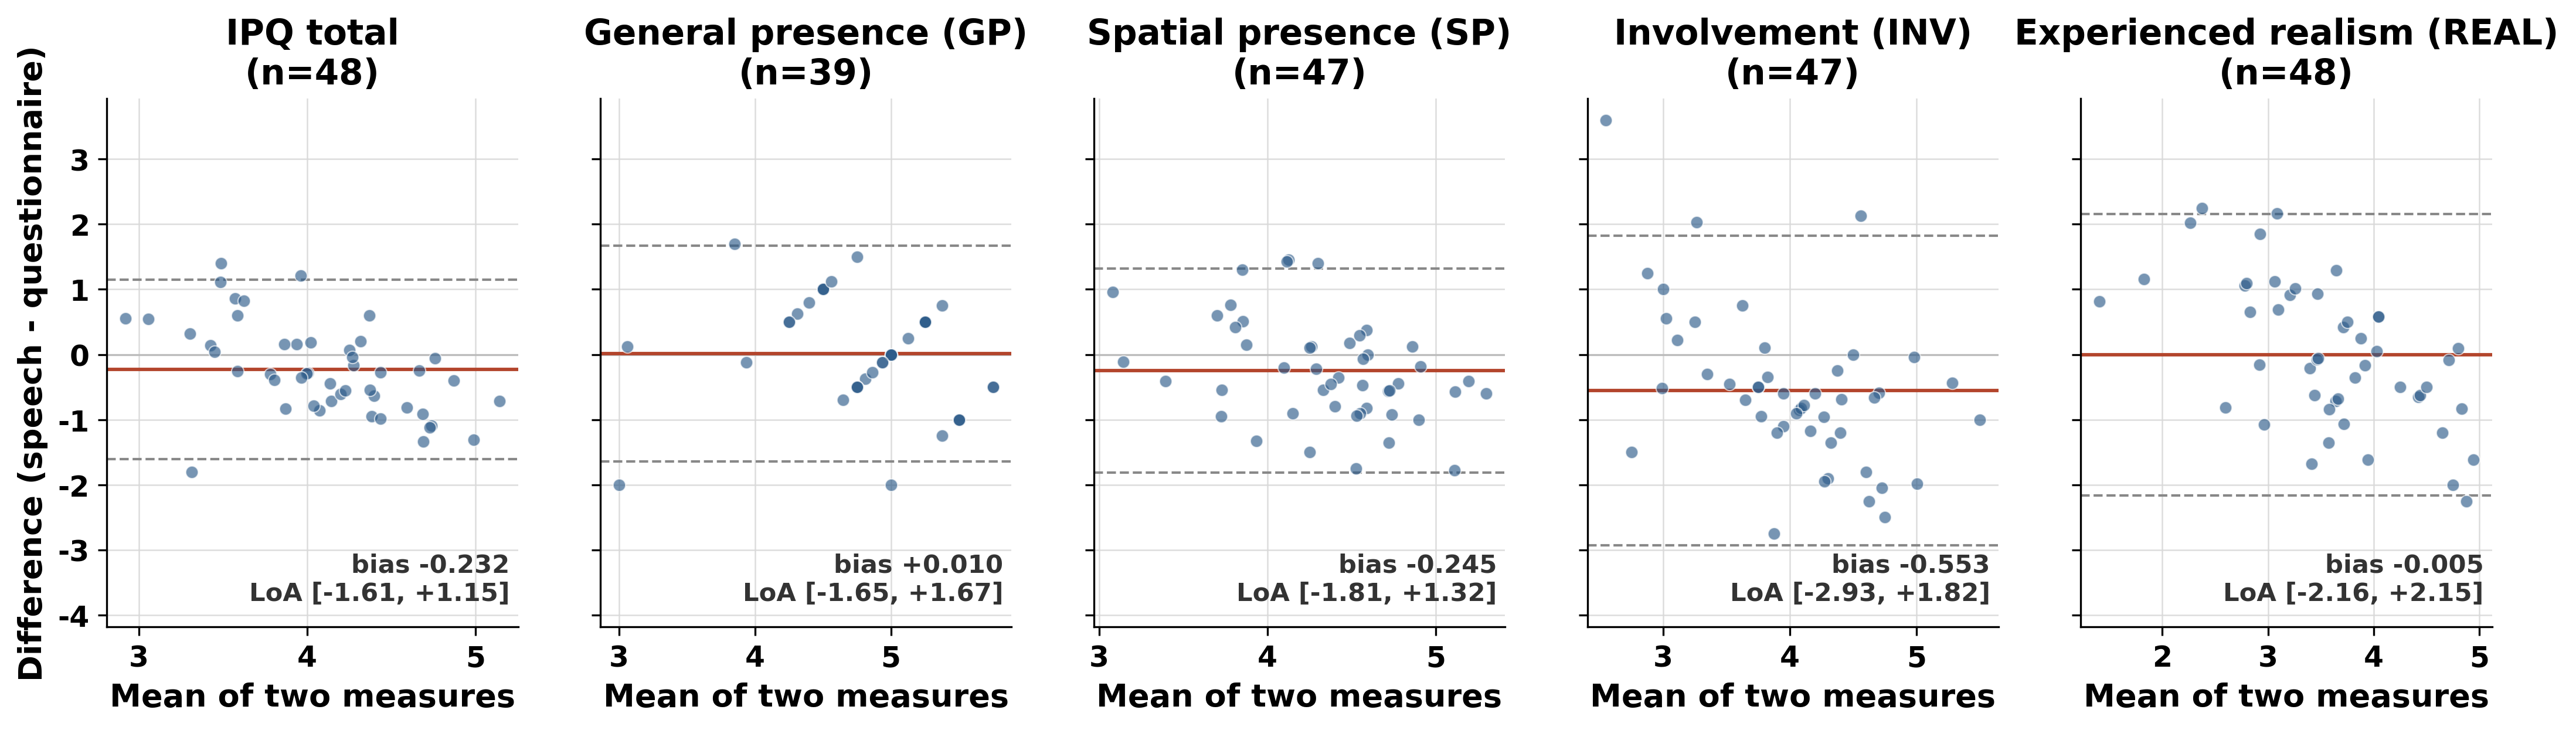
\includegraphics[width=\linewidth]{Figures/G02_bland_altman.png}
\caption{Bland--Altman plot of speech-derived vs.\ self-reported IPQ scores by construct. Mean bias and 95\% limits of agreement are drawn per construct.}
\label{fig:bland_altman}
\Description{Bland-Altman scatter with per-construct bias lines and agreement bands.}
\end{figure*}

\paragraph{Equivalence within the measurement error of the questionnaire.}
The level offset, although statistically detectable, was smaller than the measurement error of the reference instrument. At the participant level the speech-derived total sat $-0.232$ points below the questionnaire total ($SE=0.095$, $n=16$, paired $t$ $p=.028$), whereas the questionnaire's own standard error of measurement, from $\alpha=.87$~\cite{schwind2019presence} and the between-participant $SD$ of $0.579$ in the 32-participant sample, was $SEM=0.209$, giving a smallest detectable change of $SDC=0.579$. Against this margin the two totals were statistically equivalent (TOST $p=.001$), and equivalence also held under the stricter $1.96\,SEM$ margin of $\pm0.409$ ($p=.041$), under our own-sample $\alpha$ of $.816$ ($\pm0.486$, $p=.009$; $\pm0.688$, $p<.001$), and under the SDC computed from the TAP-only $SD$ ($\pm0.426$, $p=.029$). The one combination that failed was the strictest, TAP-only $SD$ with the $1.96\,SEM$ rule ($\pm0.302$, $p=.237$); Table~\ref{tab:equivalence} lists all combinations. An item-level mixed model with crossed random effects for participant and item, which accommodates the participant-specific pattern of missing items directly, estimated the method effect at $-0.297$ (90\% CI $[-0.411, -0.183]$; 458 item pairs), inside the SDC margin and touching the $1.96\,SEM$ bound. Equivalence held for every subscale under the same rules (SP $p=.002$, INV $p=.027$, REAL $p<.001$ at $1.96\,SEM$), but the subscale margins are wide because subscale reliability is lower, so we do not treat the subscale results as independent evidence.

Equivalence of means did not extend to interchangeability of individual scores. The 95\% limits of agreement for sessions were $[-1.609, +1.146]$, wider than the questionnaire's SDC, and Lin's concordance correlation was $.339$ at the session level and $.368$ at the participant level. Read against the percentile norms compiled from two decades of IPQ studies~\cite{tran2024ipq}, the group means fell in adjacent classes (questionnaire $1.20$, ``Very High''; speech $0.97$, ``High'' on the $-3$ to $+3$ metric); four of the 16 participants were classified identically by the two measures and 14 within one class, and in 11 of the 12 mismatches the speech-derived class was the lower one.

Applying the INV-side calibration term ($+0.5535$) to INV item scores and re-aggregating changes the level indicators of the total while leaving the within-person direction indicators of the total essentially unchanged (Table~\ref{tab:calibration_prepost} and Figure~\ref{fig:calibration_bias}; the participant sample size shrinks from $16$ to $15$ under the calibration input file because one participant is dropped for having fewer than three fully covered games). The mean speech--survey level offset on the total moved from $-0.221$ to $-0.134$ (pre-post reduction $=0.087$; the pre-calibration figure differs from the $-0.232$ reported above because it is computed on these 15 participants), the mean absolute error from $0.603$ to $0.584$, and the fraction of sessions within $\pm0.5$ from $45\%$ to $49\%$; the fraction of sessions with speech below survey moved from $64\%$ to $60\%$. On INV, the offset moved from $-0.554$ to $-0.000$ and the mean absolute error from $1.070$ to $0.845$. As expected for an additive constant applied within participants, the within-participant top-1, pairwise, and complete-rank rates for INV were unchanged by calibration; the top-1 and pairwise rates for the total moved slightly ($67\%\rightarrow60\%$ top-1 on the $n=15$ sub-sample; $77\%\rightarrow72\%$ pairwise). One session crossed the $6.0$ ceiling under calibration. We report both the uncalibrated and the calibrated numbers here, and keep the uncalibrated primary indicator for the direction analyses in Section~\ref{subsec:rq1_within}.

\begin{figure}[t]
\centering
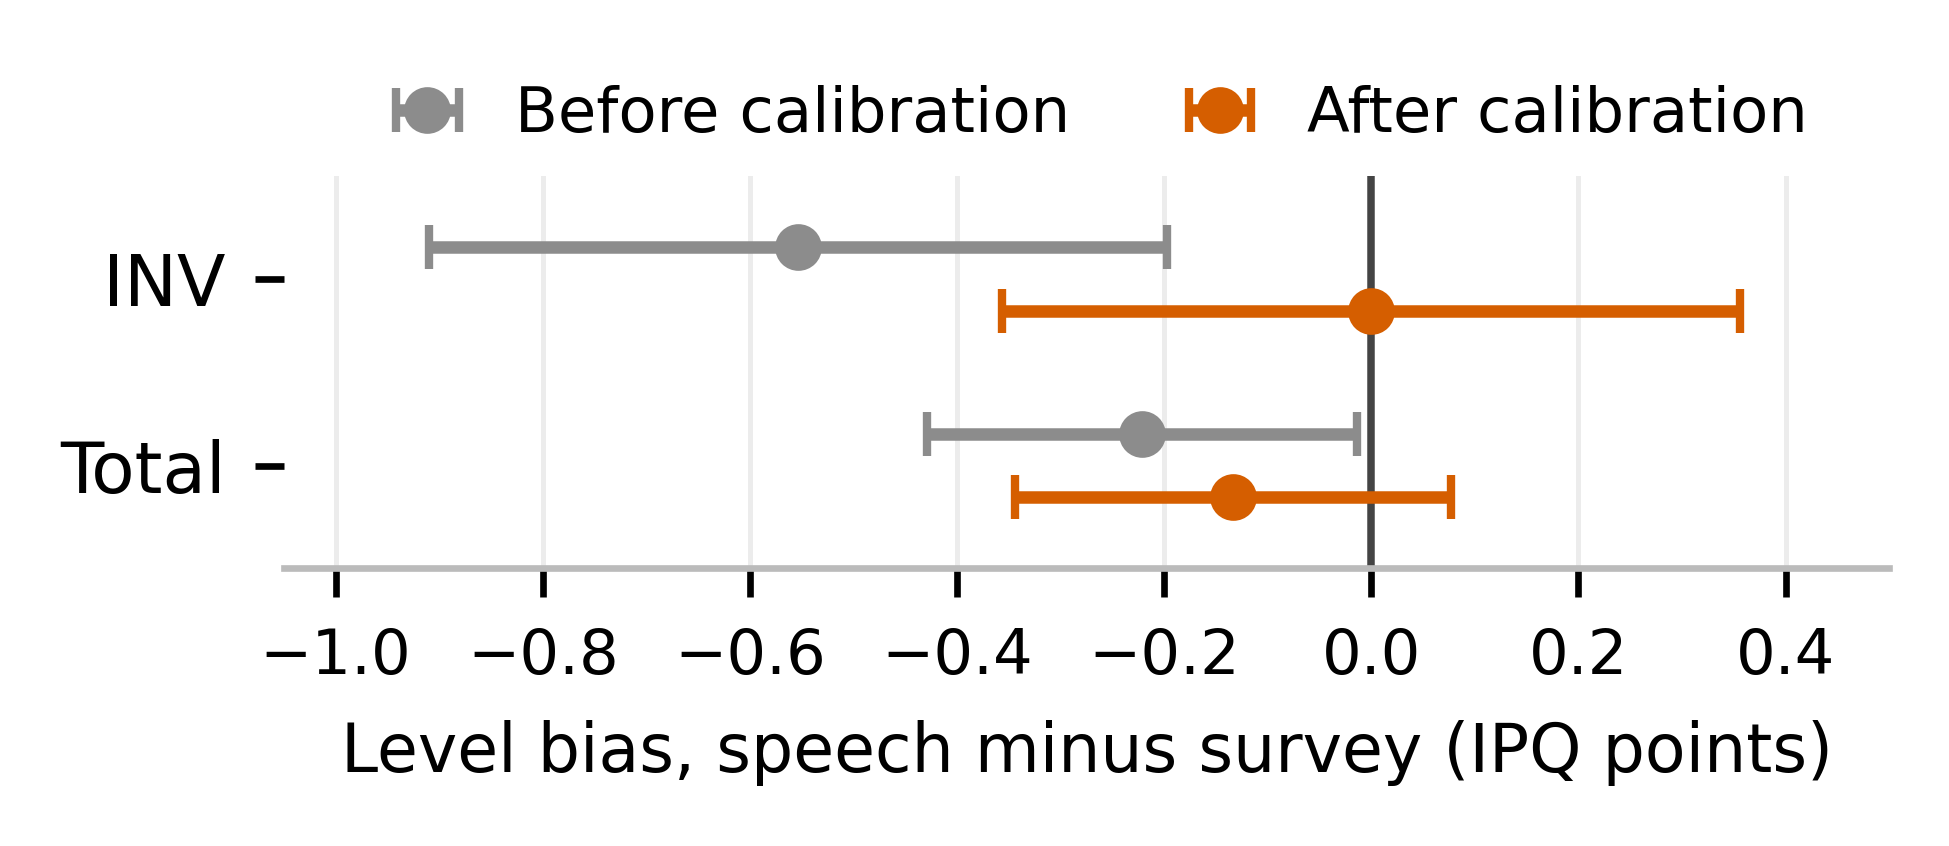
\includegraphics[width=0.5\linewidth]{Figures/F07_calibration_bias.png}
\caption{Level offset (speech minus survey) on the involvement subscale and on the total, before and after the INV-side calibration. Points are means with 95\% confidence intervals over the 47 sessions that carry a calibrated value.}
\label{fig:calibration_bias}
\Description{Horizontal interval plot comparing the mean level offset before and after calibration for the involvement subscale and the total.}
\end{figure}

Neither the amount of speech nor the amount of extracted evidence predicted the resulting score. Within the TAP sessions, the number of utterances was unrelated to the number of evidenced items ($r=+.126$, $p=.394$), to the speech-derived total ($r=+.074$, $p=.619$), and to the self-reported total ($r=+.074$, $p=.618$). The number of evidenced items was likewise unrelated to the speech-derived total ($r=+.180$, $p=.222$) and to the speech--survey level offset ($r=+.043$, $p=.771$).

Restricting the score to items backed by evidence changed almost nothing relative to scoring every item. The primary-indicator total differed from the all-item variant by $+0.018$ on average (mean absolute difference $0.093$, maximum $0.490$); the largest subscale movement was again INV ($-0.046$; mean absolute difference $0.191$, maximum $0.888$), while GP was identical and REAL differed by $+0.007$.


\subsection{Reliability of Speech Scoring (Human-Coder Reference)}
\label{subsec:rq1_reliability}

Automated scoring is judged against the agreement between independent human raters, which bounds what a scorer modeled on human judgment can reach~\cite{williamson2012framework}. To obtain this reference, two coders uninvolved in the pipeline design scored 12 of the 48 TAP sessions (four sessions from the two participants whose speech-derived and self-reported top games disagreed, PT013 and PT001, plus eight game-stratified random draws) from the raw transcripts, blind to video, survey, and pipeline output, under the pipeline's evidence rule: for each of the 14 IPQ items, whether evidence was present and, if so, a 0--6 score. Coders received the item definitions, evidence rule, and worked examples given to the LLM rater but not its norm-referenced intensity bands, so coder--LLM agreement does not reflect a shared intensity calibration.

The two coders agreed on whether evidence was present in 81\% of the 168 item slots (Cohen's $\kappa=.39$) and, where both scored, reached a quadratic weighted $\kappa$ of $.39$ and an ICC(2,1) of $.42$ at the item level. The pipeline's agreement with each coder fell within $.10$ of this human ceiling (QWK $.42$ and $.37$; ICC $.44$ and $.38$), which meets the relative criterion of Williamson et al.~\cite{williamson2012framework} but not their absolute threshold of $.70$, a level the coders themselves did not reach. Treated as a third rater on the 99 slots all three scored, the pipeline deviated least from the other two (mean deviation $-0.46$ vs.\ $+0.99$ and $-0.53$) and left inter-rater ICC unchanged ($.42 \to .42$). At the session level, however, agreement dropped (coder--coder QWK $.28$ vs.\ coder--pipeline $.06$ and $-.02$), a divergence we return to below.

The divergence has two identifiable sources. One is rater level: one coder scored about one point above both the other coder ($+1.01$) and the pipeline ($+0.99$), whereas the other coder and the pipeline agreed on level ($-0.00$), so the apparent human--machine gap is largely one rater's calibration. The other is evidence detection. Across the 168 slots the pipeline found no evidence in 33\%, close to the share in which neither coder did (29\%), but the disagreements were one-sided: 40 slots were evidenced by a coder and missed by the pipeline against one the reverse, concentrated on INV1 (missed in 12 of 12 sessions by the pipeline, 4 by both coders), INV3 (11 vs.\ 2), INV2, and REAL4. Section~\ref{sec:discussion} traces this pattern to the aggregation rule for absence-scored items.

\subsection{RQ2: Front-End Classification and Pipeline Reach}
\label{subsec:rq2}

RQ2 concerns the locally fine-tuned front-end routing classifier, which sorts each utterance into one of five categories (GP, SP, INV, REAL, NONE) before any scoring takes place. It does not itself produce IPQ scores, so it is evaluated on classification and on how far the utterances it selects travel through the pipeline, not on score accuracy.

On a held-out set of 73 multi-label utterances, the deployed configuration (the fine-tuned adapter combined with the keyword layer) reached a macro $F_1$ of $0.567$; the adapter alone reached $0.400$. Per-category results are given in Table~\ref{tab:gate} and visualized in Figure~\ref{fig:ellm_holdout}. Recall was highest for NONE ($.930$) and INV ($.650$) and lowest for SP ($.462$); the confidence intervals for GP and REAL span most of the unit interval because only four and six held-out instances were available for those categories.

\begin{table}[t]
\centering
\caption{Held-out classification performance of the deployed front end (adapter combined with keyword layer), 73 multi-label utterances. Recall is reported with Wilson 95\% confidence intervals.}
\label{tab:gate}
\small
\begin{tabular}{lcccc}
\hline
Category & $n$ & Recall & 95\% CI & Precision \\
\hline
GP & 4 & $.500$ & $[.150,\ .850]$ & $.667$ \\
SP & 13 & $.462$ & $[.232,\ .709]$ & $.857$ \\
INV & 20 & $.650$ & $[.433,\ .819]$ & $.684$ \\
REAL & 6 & $.500$ & $[.188,\ .812]$ & $.375$ \\
NONE & 43 & $.930$ & $[.814,\ .976]$ & $.833$ \\
\hline
\end{tabular}
\end{table}

\begin{figure}[t]
\centering
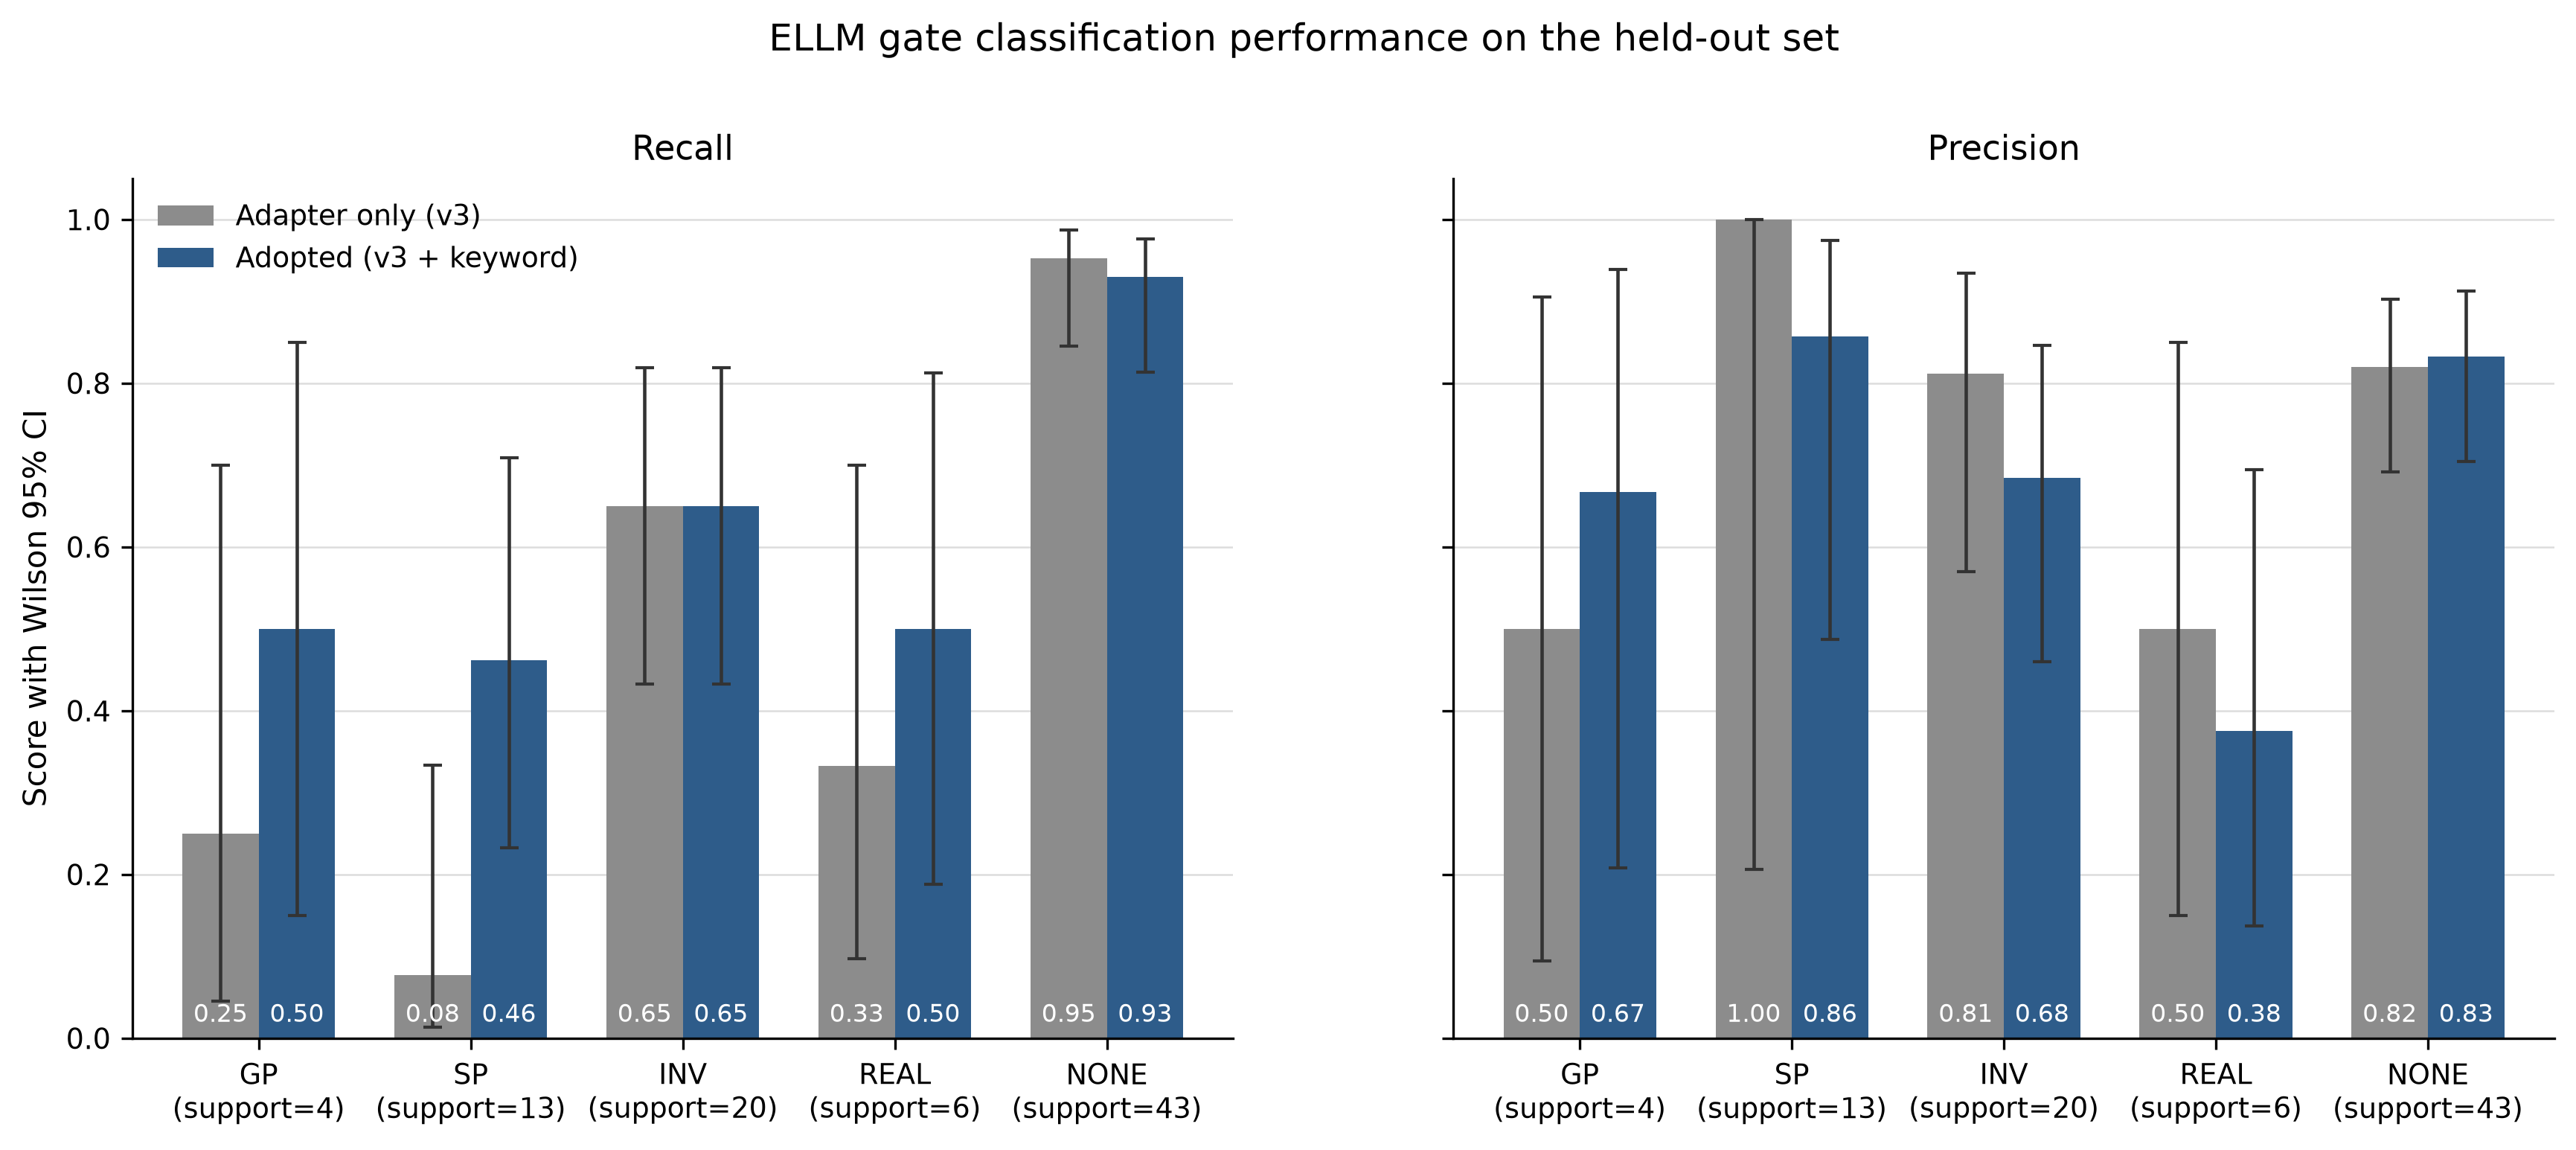
\includegraphics[width=0.85\linewidth]{Figures/G14_ellm_holdout.png}
\caption{Front-end classifier held-out recall and precision per category (Wilson 95\% CIs on recall). Adapter alone vs.\ adapter + keyword layer.}
\label{fig:ellm_holdout}
\Description{Bar chart of recall and precision per IPQ category on the held-out set.}
\end{figure}

Decomposing the two layers shows that the keyword layer buys recall at the cost of precision. Relative to the adapter alone, it raised recall for SP by $+.385$, GP by $+.250$, and REAL by $+.167$, left INV unchanged, and lowered NONE by $-.023$; precision fell for SP ($-.143$), INV ($-.128$), and REAL ($-.125$). A retrained adapter was evaluated against the deployed one and not adopted, as it lost SP recall ($-.077$) and produced a lower combined macro $F_1$ ($0.492$ vs.\ $0.567$).

Pipeline reach was measured on the 21 sessions for which the full audit was run (Figure~\ref{fig:reach_funnel}). Of the 294 item slots (14 items $\times$ 21 sessions), 289 received at least one candidate row. Of the 1{,}985 candidate rows that reached the scoring stage, 843 ($42.5\%$) were assigned a score, and 823 of those 843 passed the evidence gate into the primary indicator. Of the 92 item cells that remained empty, 87 were lost at the scoring stage; only 5 were lost at routing or at the evidence gate. A targeted keyword expansion recovered $12$ of $12$ missed INV utterances and $15$ of $19$ missed SP utterances.

\begin{figure}[t]
\centering
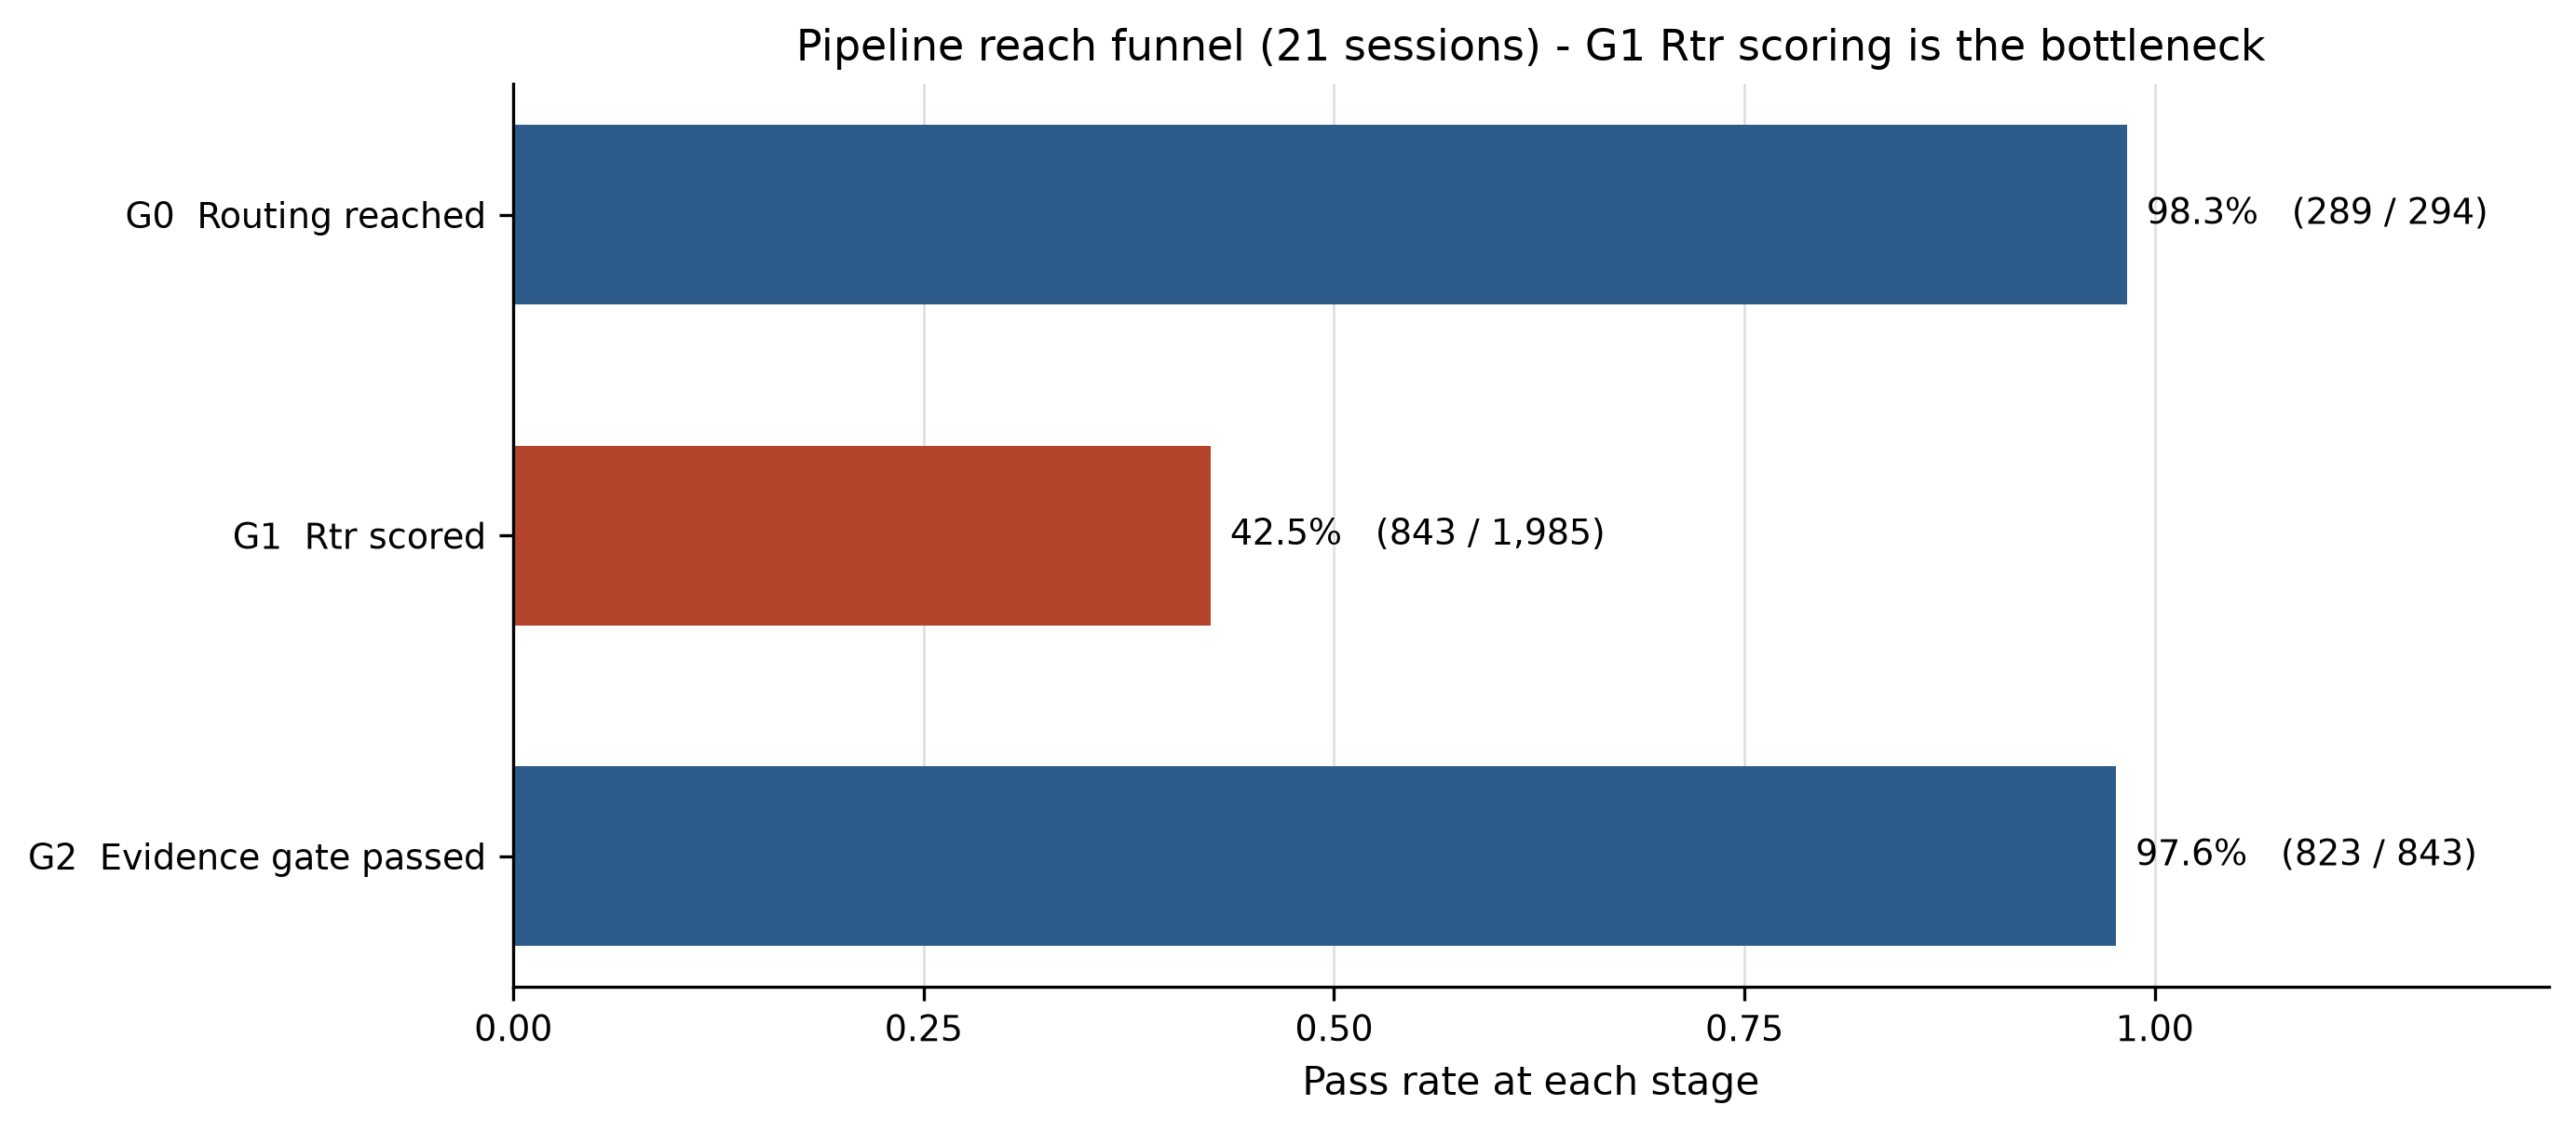
\includegraphics[width=0.85\linewidth]{Figures/G15_reach_funnel.png}
\caption{Pipeline reach funnel over the 21-session audit: candidate rows, scored items, and items that passed the evidence gate.}
\label{fig:reach_funnel}
\Description{Funnel chart from candidate rows through scored items to gate-passed items.}
\end{figure}


\subsection{Component Ablations and Negative Results}
\label{subsec:ablation}

Three components were evaluated in isolation during development and several alternatives were discarded; we report both because they locate where the pipeline's behavior comes from and where it does not.

\paragraph{Construct ontology and relation graph.}
Each of the 14 IPQ items is represented by a card (sub-indicators, boundary rules against neighboring items, and a guide paragraph), and the cards are linked by a relation graph of 62 typed edges, most of them routing edges that send a cue back to the item it belongs to. The drafter receives the cards, and the drafter and reviewer prompts receive a relation hint for the item under consideration. During development the ontology was tuned against a gold set of 65 utterances with known item assignments, using a retrieval harness as a coverage test; seven refinement steps raised gold recall from $.708$ to $1.000$. The harness is a development instrument, not the deployed routing (Section~\ref{subsec:rq2}), and the gold set is small (3--8 utterances per item), so this is a coverage check, not a precision estimate.

\paragraph{End-to-end ablation of the ontology on 12 sessions.}
A scoring-stage ablation was run on 12 sessions (four participants $\times$ three games, 894 utterances). The ablated condition emptied the item cards (names, keywords, guide text, learned examples) and removed all 62 relation edges while keeping the sub-indicator skeleton that generates the scoring cells; the deployed front-end output was reused upstream, so the comparison covers the scoring stage only. Two side effects are noted: the number of drafter calls was unchanged, and removing the guides disabled the improvement-path switch, so the ablated condition also differs by that routing change.

Session-level agreement with the questionnaire fell: the correlation with the total dropped from $r=.712$ to $.484$, mean absolute error rose from $0.517$ to $0.676$, and the within-participant top-1 match fell from 2 to 1 of the four participants (Table~\ref{tab:ablation_ontoC}).

The ablation also locates where the layer acts. Individual ratings were largely preserved: across the 442 cells scored under both conditions, $92.1\%$ of paired scores agreed within $0.5$ scale points ($48.6\%$ identical; mean signed difference $+0.03$). What moved was the assignment of evidence to items: of the 168 item slots, 123 carried evidence in the deployed condition and 109 under ablation, with SP falling from 51 to 28 and INV rising from 16 to 31. The subscale that lost the most slots is also the one whose correlation moved most (SP, $.053 \rightarrow -.320$), whereas REAL, which kept most of its slots, was unchanged ($.806 \rightarrow .798$). Because the session score is a mean over evidenced items, the layer's contribution on this evidence lies in evidence-to-item attribution, not in the severity of individual ratings.

The INV level offset was almost unchanged ($-0.742 \rightarrow -0.714$), consistent with the INV gap arising outside the rating of individual cells (Section~\ref{sec:discussion}). Four limits apply: the ablation is confined to the scoring stage; condition A is the deployed run, not a fresh replicate, so rater stochasticity is not separated from the gap; card content and relation edges were removed together, so their contributions cannot be credited separately; and with $n=12$ the values are descriptive, and GP and SP correlations were already near zero in the deployed condition, so their change of sign is not evidence that a working signal was lost.
\begin{table}[t]
\centering
\caption{End-to-end scoring-stage ablation of the construct ontology and relation graph on 12 sessions (four participants $\times$ three games; 894 utterances; 168 item slots). Condition A is the deployed run; condition C empties the card content and removes all 62 relation edges, retains the sub-indicator skeleton, and reuses the 1-Rvr output upstream. Correlations, errors, and level offsets are against the participant questionnaire; evidence slots count item slots carrying at least one piece of supporting evidence. The GP row is computed on the 11 sessions carrying GP evidence in both conditions; all other rows use 12. Cell-level agreement (442 paired cells) is reported in the text. Values are descriptive; no significance tests are reported at $n=12$.}
\label{tab:ablation_ontoC}
\small
\begin{tabular}{lrrr}
\hline
Measure & A & C & $\Delta$ \\
\hline
Session $r$ vs.\ questionnaire, total & $.712$ & $.484$ & $-.228$ \\
\quad GP & $.019$ & $-.502$ & $-.521$ \\
\quad SP & $.053$ & $-.320$ & $-.373$ \\
\quad INV & $.579$ & $.643$ & $+.064$ \\
\quad REAL & $.806$ & $.798$ & $-.008$ \\
Mean absolute error, total & $0.517$ & $0.676$ & $+0.159$ \\
Level offset, INV & $-0.742$ & $-0.714$ & $+0.028$ \\
Top-1 game match (of 4 participants) & $2$ & $1$ & $-1$ \\
Evidence slots, SP (of 60) & $51$ & $28$ & $-23$ \\
Evidence slots, INV (of 48) & $16$ & $31$ & $+15$ \\
Evidence slots, REAL (of 48) & $45$ & $39$ & $-6$ \\
Evidence slots, GP (of 12) & $11$ & $11$ & $0$ \\
\hline
\end{tabular}
\end{table}

\paragraph{Keyword layer in the front-end classifier.}
On the 73-utterance hold-out set, adding a keyword layer to the fine-tuned classifier raised SP recall from $.077$ to $.462$ at a precision cost from $1.000$ to $.857$ and GP recall from $.250$ to $.500$, while INV recall stayed at $.650$ (Figure~\ref{fig:ellm_holdout}); exact-set agreement was $.726$ for both variants. An error analysis of 31 missed utterances found the classifier accounting for most INV detections and the keyword layer for all SP detections, so the two layers cover different constructs.

\paragraph{What did not work.}
Interventions at the scoring stage repeatedly failed to improve agreement with the questionnaire. Injecting empirical anchors into the rater prompt worsened every metric on a paired check (quadratic-weighted $\kappa$ $.188\rightarrow.136$) and was reverted. Assigning maximal scores to exclamatory utterances left the INV4--questionnaire correlation unchanged ($.056\rightarrow.045$). Replacing mean with max aggregation halved the INV offset ($-1.144\rightarrow-0.500$) without recovering rank agreement ($r$ $.047\rightarrow.021$), and dropping the least-covered INV items widened the offset ($-0.554\rightarrow-0.641$ and $-0.710$). Projecting embeddings onto construct axes failed for the full item set because of synonym overlap among the realism items, and nearest-neighbor example injection had no measurable effect. These failures showed that the INV gap was not in the rater; the human-coder comparison later located it at the aggregation gate (Section~\ref{sec:discussion}).


\subsection{RQ3: Effect of the Think-Aloud Protocol on Reported Presence}
\label{subsec:rq3}

Table~\ref{tab:group} and Figure~\ref{fig:group_forest} contrast the two groups on the five IPQ measures. The TAP group reported higher presence on the IPQ total ($+0.441$, $t(26.2)=2.294$, $p=.030$, $d=0.81$), with the largest subscale difference on INV ($+0.656$, $t(30.0)=2.104$, $p=.044$, $d=0.74$). After Holm--Bonferroni correction across the five measures, none of the differences remained significant (IPQ total $p_{\mathrm{Holm}}=.150$; INV $p_{\mathrm{Holm}}=.176$). The effect size for the IPQ total was Hedges' $g=0.791$, 95\% CI $[0.086,\ 1.495]$, with a lower bound only marginally above zero. The think-aloud instruction did not raise workload: the TAP group's RTLX ($40.2$) did not differ detectably from the non-TAP group's ($35.1$; $p=.415$), and no individual TLX item differed either (Table~\ref{tab:workload}, all $p \geq .15$). Nor did it lower presence: the TAP group's IPQ total was higher, not lower, than the non-TAP group's.

\begin{table}[t]
\centering
\caption{Group comparison on participant-level means (Welch's $t$-test, $n=16$ per group). Asterisks mark uncorrected $p<.05$; no measure remains significant after Holm--Bonferroni correction across the five measures.}
\label{tab:group}
\small
\begin{tabular}{lccccccc}
\hline
Measure & TAP $M$ ($SD$) & non-TAP $M$ ($SD$) & Diff & $t$ & $p$ & $p_{\mathrm{Holm}}$ & $d$ \\
\hline
IPQ total & $4.202$ ($0.427$) & $3.762$ ($0.639$) & $+0.441$ & $2.294$ & $.030$* & $.150$ & $0.81$ \\
GP & $4.833$ ($0.621$) & $4.271$ ($1.097$) & $+0.562$ & $1.785$ & $.087$ & $.261$ & $0.63$ \\
SP & $4.471$ ($0.408$) & $4.229$ ($0.836$) & $+0.242$ & $1.039$ & $.310$ & $.310$ & $0.37$ \\
INV & $4.323$ ($0.883$) & $3.667$ ($0.881$) & $+0.656$ & $2.104$ & $.044$* & $.176$ & $0.74$ \\
REAL & $3.589$ ($0.583$) & $3.146$ ($0.821$) & $+0.443$ & $1.759$ & $.090$ & $.261$ & $0.62$ \\
\hline
\end{tabular}
\end{table}

\begin{table}[t]
\centering
\caption{Workload by group: NASA-TLX items and RTLX (0--100; participant-level means over the three games; Welch's $t$-test, $n=16$ per group). Asterisks mark uncorrected $p<.05$; $p_{\mathrm{Holm}}$ is corrected across the seven rows.}
\label{tab:workload}
\small
\begin{tabular}{lcccccc}
\hline
Measure & TAP $M$ ($SD$) & non-TAP $M$ ($SD$) & Diff & $t$ & $p$ & $p_{\mathrm{Holm}}$ \\
\hline
Mental demand & $34.6$ ($23.2$) & $28.1$ ($19.3$) & $+6.5$ & $.86$ & $.398$ & $1.000$ \\
Physical demand & $37.5$ ($24.8$) & $32.5$ ($22.6$) & $+5.0$ & $.60$ & $.555$ & $1.000$ \\
Temporal demand & $31.2$ ($22.9$) & $29.8$ ($21.8$) & $+1.5$ & $.18$ & $.855$ & $1.000$ \\
Performance & $52.5$ ($18.8$) & $43.8$ ($19.6$) & $+8.8$ & $1.29$ & $.208$ & $1.000$ \\
Effort & $58.5$ ($17.3$) & $48.8$ ($20.5$) & $+9.8$ & $1.46$ & $.155$ & $1.000$ \\
Frustration & $26.9$ ($21.3$) & $27.7$ ($22.8$) & $-0.8$ & $-0.11$ & $.916$ & $1.000$ \\
RTLX & $40.2$ ($16.6$) & $35.1$ ($18.3$) & $+5.1$ & $.83$ & $.415$ & $1.000$ \\
\hline
\end{tabular}
\end{table}

\begin{figure*}[t]
\centering
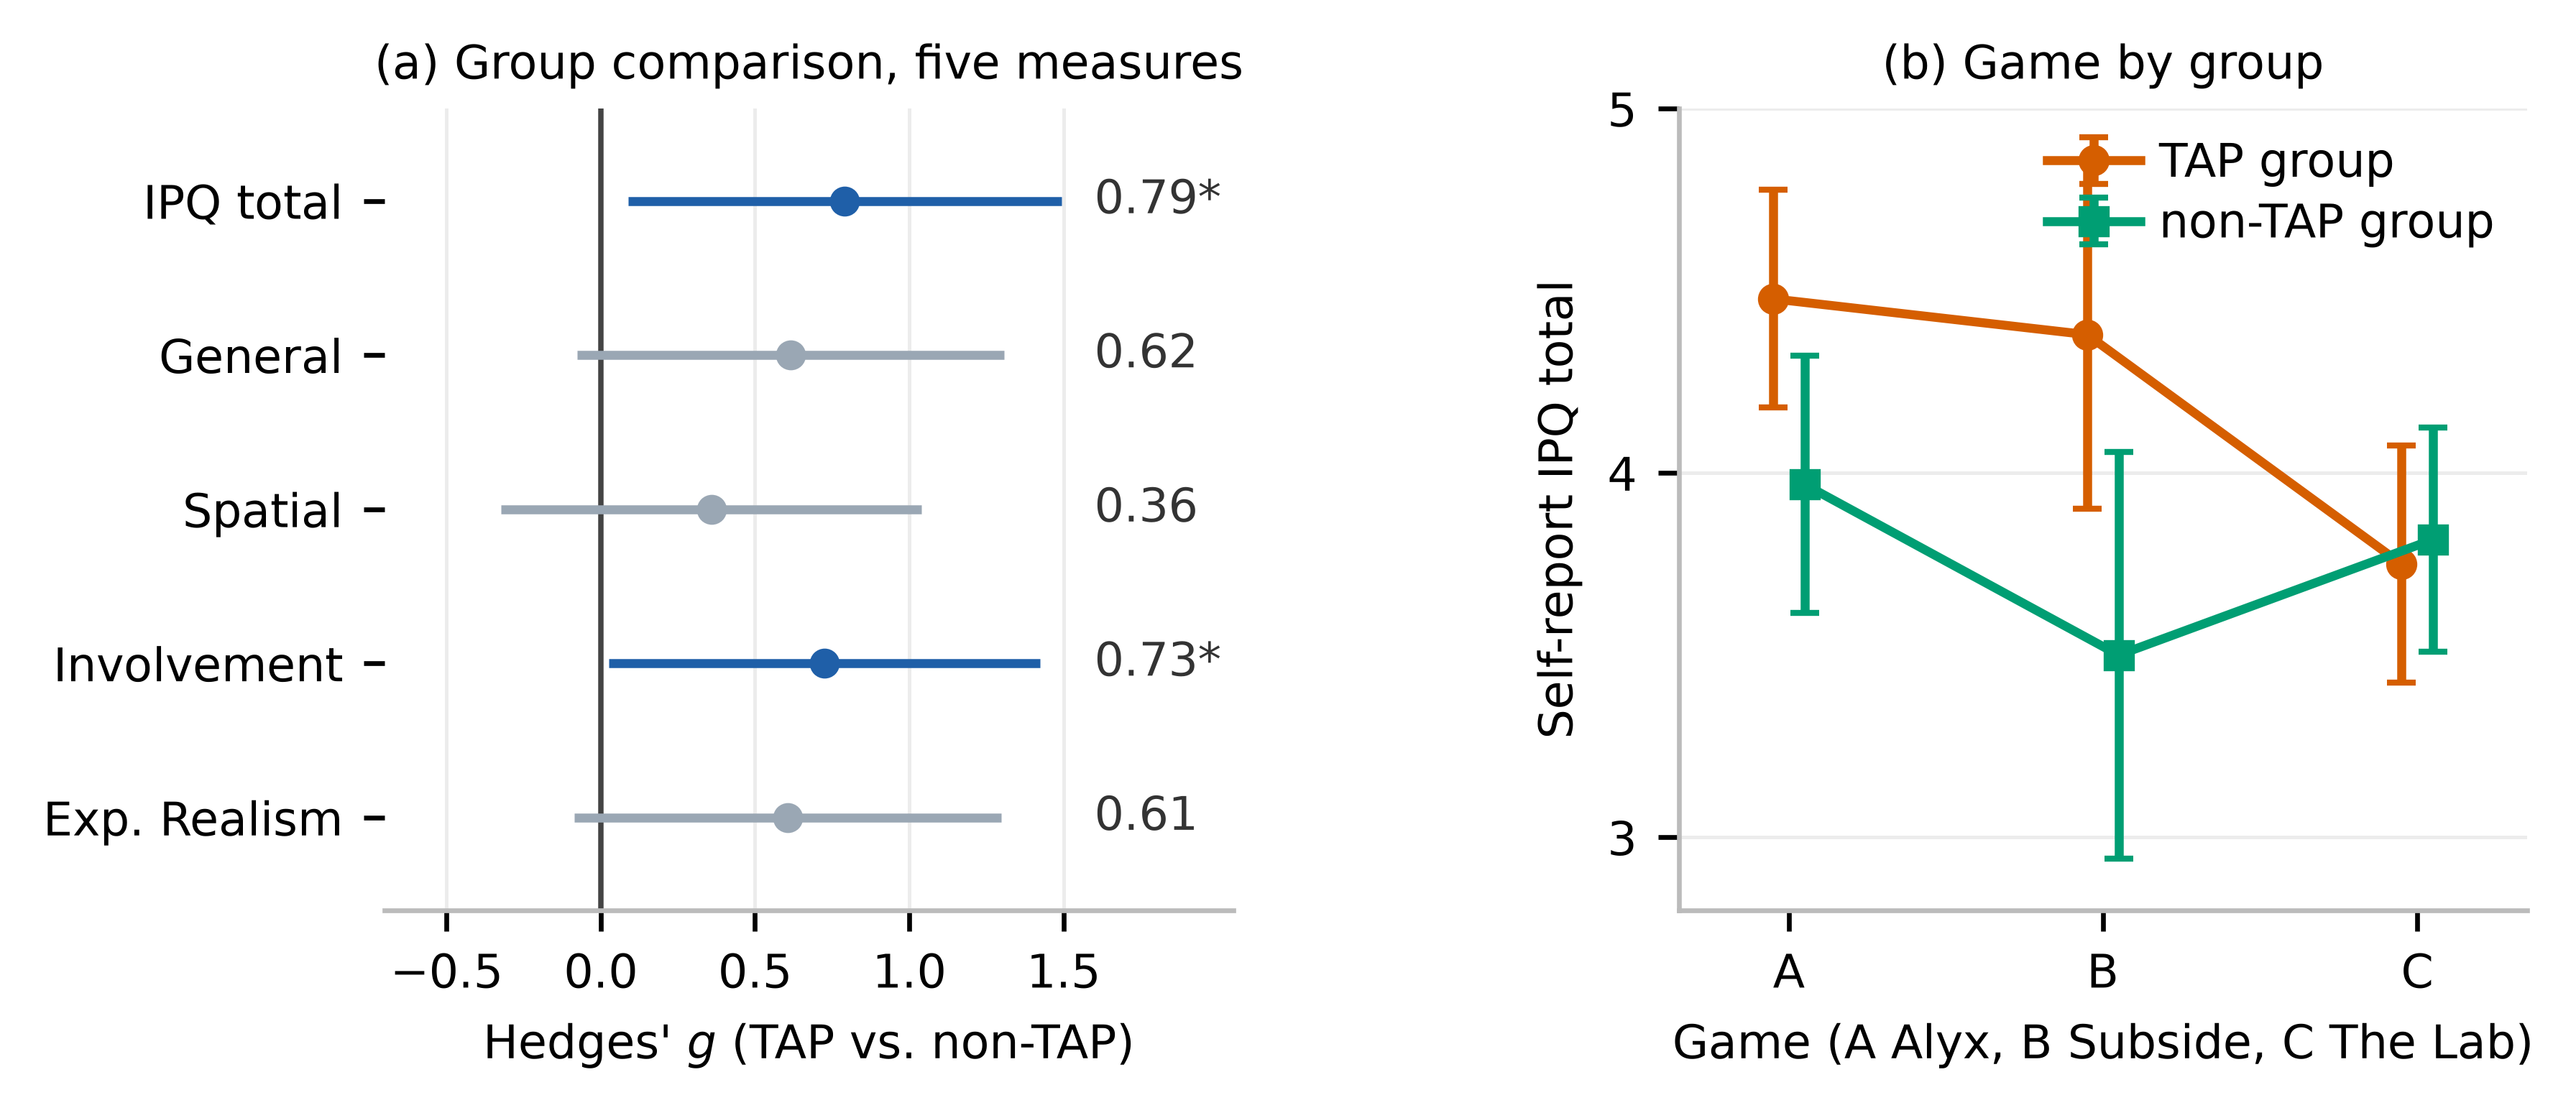
\includegraphics[width=0.76\textwidth]{Figures/F10_11_rq3_pair.png}
\caption{Group comparison on the five IPQ measures (a) and the game by group pattern on the self-reported IPQ total (b). 
In (a), each row is Hedges' $g$ with its 95\% confidence interval and the value at the right is that effect size; asterisks mark uncorrected $p<.05$, no measure remains significant after Holm--Bonferroni correction across the five measures, and both $p$ values are given in Table~\ref{tab:group}. In (b), points are group means with 95\% confidence intervals ($n=16$ per group).}
\Description{Two square panels side by side. The left panel is an interval plot of five standardized group differences with a zero reference line. The right panel plots self-reported IPQ totals for the two groups across the three VR games with confidence intervals.}
\label{fig:group_forest}
\end{figure*}

Two observations qualify the group difference. First, the TAP group scored higher on every measure, and on workload (Table~\ref{tab:workload}), so a general response-intensity difference cannot be separated from a presence-specific effect with these data. 
Second, the difference was not uniform across games (Figure~\ref{fig:group_forest}): at the session level it was present for Alyx ($+0.509$, $p=.026$) and Subside ($+0.879$, $p=.016$) but absent for The Lab ($-0.067$, $p=.753$).



Assignment and order were balanced. Stratification by motion-sickness susceptibility and prior VR experience was fully balanced across the two groups (4/4/4/4 per cell), with no group difference in susceptibility scores ($p=.822$) and no imbalance in game-order assignment ($\chi^2$ $p=.693$). A test for order effects across the three session positions was null ($p=.945$). Entering stratum, game order, and susceptibility as covariates in a participant-level regression left the coefficient essentially unchanged ($+0.440 \rightarrow +0.411$) while moving the $p$ value to the boundary ($.029 \rightarrow .052$) with 24 residual degrees of freedom.

Three data anomalies were identified from the session logs: one non-TAP participant ran the second game with passthrough enabled, one non-TAP participant completed the workload questionnaire from recall on the following day, and one non-TAP participant executed a game order different from the assigned one. Excluding the first two in a sensitivity analysis left the result unchanged ($+0.441 \rightarrow +0.422$, $p=.030$).

Independently of group, the three games differed in reported presence (Table~\ref{tab:game}). Alyx yielded the highest IPQ total and The Lab the lowest, with the Alyx--The Lab contrast the only reliable pairwise difference ($+0.440$, $t(31)=3.516$, $p=.001$). The game difference was carried by SP and REAL, on both of which Alyx exceeded The Lab ($p<.001$), whereas INV did not differ across games.

\begin{table}[t]
\centering
\caption{Self-reported IPQ total and subscales by game, both groups combined ($n=32$ participants; $M$ ($SD$) of participant-level scores), and paired contrasts within participants (mean difference and paired-$t$ $p$, $df=31$; $t$ values in the accompanying CSV). Asterisks mark uncorrected $p<.05$.}
\label{tab:game}
\small
\begin{tabular}{lccc cc cc cc}
\hline
 & \multicolumn{3}{c}{$M$ ($SD$)} & \multicolumn{2}{c}{Alyx $-$ Subside} & \multicolumn{2}{c}{Alyx $-$ The Lab} & \multicolumn{2}{c}{Subside $-$ The Lab} \\
Scale & Alyx & Subside & The Lab & Diff & $p$ & Diff & $p$ & Diff & $p$ \\
\hline
Total & $4.22$ ($0.66$) & $3.94$ ($1.06$) & $3.78$ ($0.59$) & $+0.283$ & $.122$ & $+0.440$ & $.001$* & $+0.156$ & $.415$ \\
GP & $4.84$ ($1.02$) & $4.38$ ($1.39$) & $4.44$ ($1.01$) & $+0.469$ & $.007$* & $+0.406$ & $.051$ & $-0.062$ & $.813$ \\
SP & $4.66$ ($0.61$) & $4.29$ ($1.09$) & $4.10$ ($0.79$) & $+0.362$ & $.041$* & $+0.556$ & $<.001$* & $+0.194$ & $.337$ \\
INV & $4.01$ ($1.27$) & $3.79$ ($1.23$) & $4.19$ ($1.03$) & $+0.219$ & $.350$ & $-0.180$ & $.387$ & $-0.398$ & $.099$ \\
REAL & $3.74$ ($0.85$) & $3.54$ ($1.28$) & $2.82$ ($1.14$) & $+0.203$ & $.441$ & $+0.922$ & $<.001$* & $+0.719$ & $.016$* \\
\hline
\end{tabular}
\end{table}

